\documentclass{standalone}
\usepackage{tikz}
\usetikzlibrary{shapes, positioning, calc}

\begin{document}
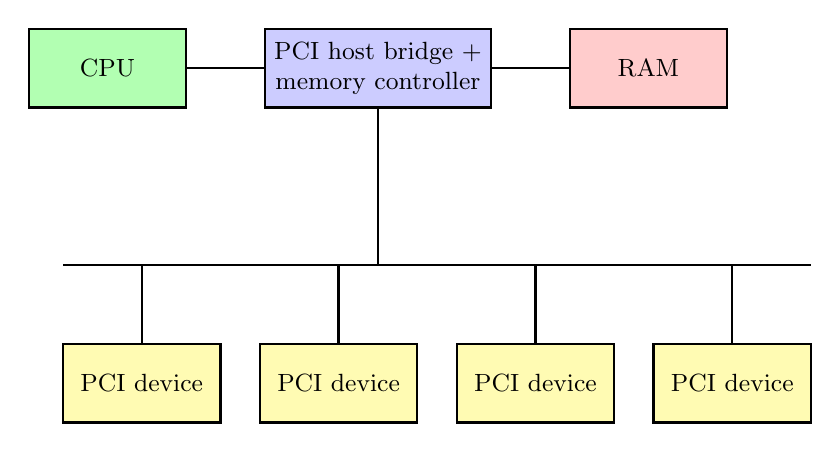
\begin{tikzpicture}

\tikzset{
    every node/.style={font=\small, minimum width=2cm, minimum height=1cm, outer sep=0pt, draw, thick, align=center},
}

% Nodes
\node[fill=green!30] (cpu) {CPU};
\node[fill=blue!20, right=1cm of cpu] (host) {PCI host bridge + \\ memory controller};
\node[fill=red!20, right=1cm of host] (ram) {RAM};

% PCI devices
\node[fill=yellow!30, below=3cm of host, xshift=-3cm] (pci1) {PCI device};
\node[fill=yellow!30, right=0.5cm of pci1] (pci2) {PCI device};
\node[fill=yellow!30, right=0.5cm of pci2] (pci3) {PCI device};
\node[fill=yellow!30, right=0.5cm of pci3] (pci4) {PCI device};

% Connections
\draw[thick] (cpu) -- (host);
\draw[thick] (ram) -- (host);

\draw[thick] (host.south) -- ++(0, -2.0);
% \draw[thick] (host) -- ++(0, -0.5) -- ++(0, -0.5) -- ++(-3.5, 0);
% \draw[thick] (host) -- ++(0, -0.5) -- ++(0, -0.5) -- ++(3.5, 0);

% PCI bus
\draw[thick] ([yshift=+1cm]pci1.north west) -- ([yshift=+1cm]pci4.north east);

% Connections from PCI bus to PCI devices
\foreach \i in {pci1, pci2, pci3, pci4}
  \draw[thick] ([yshift=+1cm]\i.north) -- (\i.north);

\end{tikzpicture}
\end{document}
